\documentclass{beamer}
\usepackage[utf8]{inputenc}
\usepackage{bm}
\usepackage{tikz}
\usepackage{amsmath}
\usetikzlibrary{arrows}

\usetheme{Madrid}
\usecolortheme{default}


%------------------------------------------------------------
%This block of code defines the information to appear in the
%Title page
\title[When Taylor Series Go Wrong] %optional
{When Taylor Series Go Wrong}

% \subtitle{A short story}

\author[H.~Han]
{H.~Han}

% \institute[VFU] % (optional)
% {
%   \inst{1}%
%   Faculty of Physics\\
%   Very Famous University
%   \and
%   \inst{2}%
%   Faculty of Chemistry\\
%   Very Famous University
% }

% \date[VLC 2021] % (optional)
% {Very Large Conference, April 2021}


%End of title page configuration block
%------------------------------------------------------------



%------------------------------------------------------------
%The next block of commands puts the table of contents at the 
%beginning of each section and highlights the current section:

% \AtBeginSection[]
% {
%   \begin{frame}
%     \frametitle{Table of Contents}
%     \tableofcontents[currentsection]
%   \end{frame}
% }
%------------------------------------------------------------


\begin{document}

%The next statement creates the title page.
\frame{\titlepage}


%---------------------------------------------------------
%This block of code is for the table of contents after
%the title page
% \begin{frame}
% \frametitle{Table of Contents}
% \tableofcontents
% \end{frame}
%---------------------------------------------------------


\section{First section}

%---------------------------------------------------------
%Changing visivility of the text
% \begin{frame}
% \frametitle{Sample frame title}
% This is a text in second frame. For the sake of showing an example.
%
% \begin{itemize}
%     \item<1-> Text visible on slide 1
%     \item<2-> Text visible on slide 2
%     \item<3> Text visible on slides 3
%     \item<4-> Text visible on slide 4
% \end{itemize}
% \end{frame}

%---------------------------------------------------------


%---------------------------------------------------------
%Example of the \pause command
% \begin{frame}
% In this slide \pause
%
% the text will be partially visible \pause
%
% And finally everything will be there
% \end{frame}
%---------------------------------------------------------

% \section{Second section}

%---------------------------------------------------------
\begin{frame}
\frametitle{Taylor Series}

\begin{block}{Taylor Series at $c$ Generated by $f$}
	Let $f$ be a function that is infinitely differentiable at $c$. Then the Taylor series of $f$ at $c$ is
	\begin{equation}
		\sum_{n=0}^{\infty} \frac{f^{(n)}(c)}{n!} (x-c)^n
	\end{equation}
\end{block}

\begin{alertblock}{\textbf{Not} All all Functions Converges to its Taylor Series}
	Obvious Cases: when $f \notin C^{\infty}$ ($f$ are not infintely differentiable) at $c$.
\end{alertblock}


% \begin{alertblock}{Important theorem}
% Sample text in red box
% \end{alertblock}
%
% \begin{examples}
% Sample text in green box. The title of the block is ``Examples".
% \end{examples}
\end{frame}

\begin{frame}
\frametitle{Taylor Theorem}

\begin{block}{Taylor's Theorem}
	The Taylor Series converges to its function $f$ at $c$ if and only if 
	\[
		\lim_{n \to \infty} \frac{f^n(x_1)}{n!}(x-c)^n = 0
	\]

	Where $x_1$ is between $c$ and $x$.
\end{block}

\end{frame}

\begin{frame}
\frametitle{An Interesting Example}

\begin{block}{Example}
	Consider function
	\[ 
		f(x) = 
		\begin{cases}
			e^{-\frac{1}{x^2}} & x \neq 0 \\
			0 & x = 0
		\end{cases}
	\]

	This function is infinitely differential at $c=0$ and $f^{(n)}(0) = 0$. Thus, the Taylor series of $f$ at $c=0$ is 0. Which is clearly wrong.
	\begin{figure}
	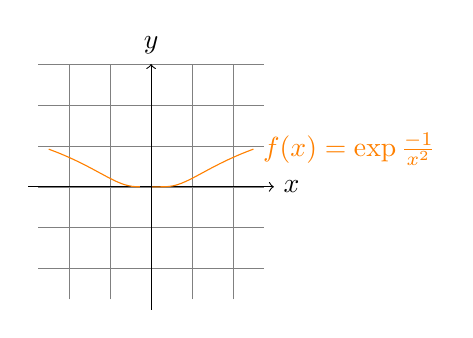
\begin{tikzpicture}[scale = 1.3,domain=-1:1]
  \draw[step=0.4, very thin,color=gray] (-1.1,-1.1) grid (1.1,1.2);

  \draw[->] (-1.2,0) -- (1.2,0) node[right] {$x$};
  \draw[->] (0,-1.2) -- (0,1.2) node[above] {$y$};


  \draw[color=orange, domain=0.01:1] plot (\x,{exp(-1/\x)}) node[right] {$f(x) = \exp{\frac{-1}{x^2}}$};
  \draw[color=orange, domain=-1:-0.11] plot (\x,{exp(1/\x)}); 
\end{tikzpicture}
\end{figure}
\end{block}

\end{frame}


%---------------------------------------------------------
%Two columns
% \begin{frame}
% \frametitle{Two-column slide}
%
% \begin{columns}
%
% \column{0.5\textwidth}
% This is a text in first column.
% $$E=mc^2$$
% \begin{itemize}
% \item First item
% \item Second item
% \end{itemize}
%
% \column{0.5\textwidth}
% This text will be in the second column
% and on a second tought this is a nice looking
% layout in some cases.
% \end{columns}
% \end{frame}
%---------------------------------------------------------


\end{document}
